\section{From Online Learning to Convex Optimization and Machine Learning}
\label{section:applications}

The results in Section~\ref{section:algorithms} immediately implies new
algorithms and results in convex optimization and machine learning. See
\cite{Orabona-2014} and \cite{Luo-Schapire-2015} for more results.

\begin{algorithm}[t]
\caption{SGD algorithm based on KT potential \label{algorithm:kt-sgd}}
\begin{algorithmic}[1]
{
\STATE{Initialize $\Wealth_0 \leftarrow 1$ and $\theta_0 \leftarrow 0$}
\FOR{$t=1,2,\dots,T$}
\STATE{Set $w_t \leftarrow \Wealth_{t-1} \tfrac{\theta_{t-1}}{t} $}
\STATE{Select an index $j$ at random from $\{1,2,\dots,N\}$ and compute $h_t \in \partial \ell_j(w_{t-1})$}
\STATE{Update $\theta_t \leftarrow \theta_{t-1} - h_t$ and $\Wealth_t \leftarrow \Wealth_{t-1} - \langle h_t, w_t \rangle$}
\ENDFOR
\STATE{Output $\overline{w}_T = \tfrac{1}{T}\sum_{t=1}^T w_t$}
}
\end{algorithmic}
\end{algorithm}

\textbf{Convex Optimization.} 
Consider an emprical risk minimization problem of the form
%
\begin{equation}
\label{equation:objective-function}
F(w) = \frac{1}{N} \sum_{i=1}^N \ell_i(w),
\end{equation}
%
where $\ell_i:\R^d \to \R$ is convex.\footnote{The algorithm can also be
implemented and analyzed with kernels~\citep{Orabona-2014}.} It is immediate to
transform Algorithm~\ref{algorithm:hilbert-space-olo} into a \ac{SGD} algorithm
for this problem. In Algorithm~\ref{algorithm:kt-sgd}, $\partial\ell_j(w)$
denotes the set of subgradients of $\ell_j$ at a point $w$.  We assume that the
norm of the subgradient of $\ell_j$ is bounded by $1$.

Beside the simplicity of the Algorithm~\ref{algorithm:kt-sgd}, it has the
important property is that it \emph{does not have a learning rate to be tuned},
yet it achieves the optimal convergence rate. If $\widehat{w} = \argmin_w F(w)$
is the optimal solution of~\eqref{equation:objective-function}, the following
theorem states the rate of convergence.
%
\begin{theorem}
The average $\overline{w}_T$ produced by Algorithm~\ref{algorithm:kt-sgd} is
an approximate minimizer of the objective function \eqref{equation:objective-function}:
\[
\Exp\left[F(\overline{w}_T)\right] - F(\widehat{w}) \leq \tfrac{\norm{\widehat{w}}}{\sqrt{T}} \sqrt{\log(1+4 T^2 \norm{\widehat{w}}^2)} +\tfrac{1}{T} \; .
\]
\end{theorem}
%
Note that in the above theorem, $T$ can be larger (multiple epochs) or smaller
than $N$.

\textbf{Machine Learning.} In machine learning, the minimization of a function
\eqref{equation:objective-function} is just a proxy to minimize the \emph{true
risk} over an unknown distribution. For example, $\ell_i(w)$ can be a
regression loss, e.g. the logistic loss, over i.i.d. samples $\{(X_i,
Y_i)\}_{i=1}^N$. That is, $\ell_i(w)=\ell(w,X_i,Y_i)$. A common approach to
have a small risk on the test set is to minimize a regularized objective
function:
%
\begin{equation}
\label{eq:reg_logloss}
F_\lambda^{\text{Reg}}(w) = \lambda \norm{w}^2 + \frac{1}{N} \sum_{i=1}^N \ell(w, X_i, Y_i) \; .
\end{equation}
%
This problem is strongly convex, so there are very efficient methods to
minimize it, hence we can assume to be able to get the minimizer of
$F_\lambda^{\text{Reg}}$ with arbitrary high precision. Yet, this is not
enough. In fact, we are rarely interested in the value of the objective
function $F_\lambda^{\text{Reg}}$ or its mimizer, rather we are interested in
the \emph{true risk} of a solution $w$, that is $\Exp[\ell(w,X,Y)]$ where $X,Y$
comes from the same \emph{unknown distribution} from which the training set
$\{(X_i,Y_i)\}_{i=1}^N$ and future test points come from. Hence, in order to
get a good performance we have to select a good regularization parameter. In
particular, from \cite{Sridharan-Shalev-Shwartz-Srebro-2009} we get
\[
\Exp[\ell(\widehat{w},X,Y)] - \Exp[\ell(w^*,X,Y)] \le O(\lambda \norm{w^*}^2 + \tfrac{1}{\lambda N}),
\]
where $w^*=\argmin_w \Exp[\ell(w,X,Y)]$ and $\widehat{w} = \argmin_w
F_\lambda^{\text{Reg}}(w)$.  From the above bound, it is clear that the optimal value
of $\lambda$ depends on the $\norm{w^*}$ that is unknown. We would like to
stress that this is not just a theoretical problem: Any practictioner knows how
painfull it is to find the right regularization for the problem at hand.
Assuming we would know $\norm{w^*}$, we could set $\lambda = O(1/(\norm{w^*}
\sqrt{N}))$ to achieve
%
\begin{equation}
\label{equation:optimal-rate}
\Exp[\ell(\widehat{w},X,Y)] - \Exp[\ell(w^*,X,Y)] \le O\left(\tfrac{\norm{w^*}}{\sqrt{N}}\right) \; .
\end{equation}

Using Algorithm~\ref{algorithm:hilbert-space-olo} with only single pass over
the dataset, we get almost the same guarantee \eqref{equation:optimal-rate}
\emph{without knowing $\norm{w^*}$, and without tuning any parameters, learning
rates, regularization parameters, etc.}
%
\begin{theorem}
Assume that $(X, Y), (X_1, Y_1), (X_2, Y_2), \dots, (X_N,Y_N)$ are i.i.d.  and
let $\ell_t(w) = \ell(w,X_t,Y_t)$. Feed
Algorithm~\ref{algorithm:hilbert-space-olo} with $g_t = - \partial
\ell_t(w_t)$. Then the average $\overline{w}_N = \frac{1}{N} \sum_{i=1}^N w_i$
of algorithm's predictions satisfies
$$
\Exp[\ell(\overline{w}_N,X,Y)] - \Exp[\ell(w^*,X,Y)] \le \frac{\norm{w^*}}{\sqrt{N}} \sqrt{\log(1+4 N^2 \norm{w^*}^2)} + \tfrac{1}{N} \; .
$$
\end{theorem}
%
Comparing this guarantee to the one in \eqref{equation:optimal-rate}, we see
that, just paying a sub-logarithmic price, we obtain the optimal convergence
rate and we remove all the parameters.

\begin{figure}[t]
\centering
\subfigure{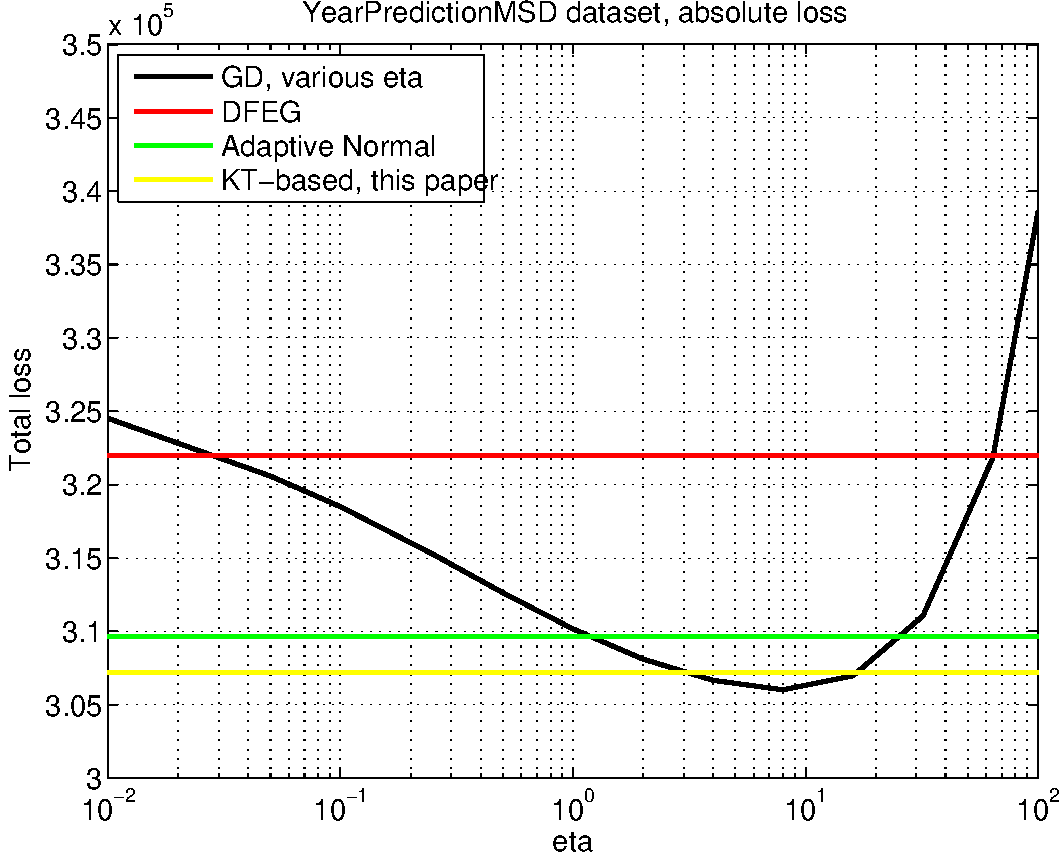
\includegraphics[width=0.32\textwidth]{../NIPS-2016-submission/figs/yearpredictionmsd_kt-crop.pdf}}
\subfigure{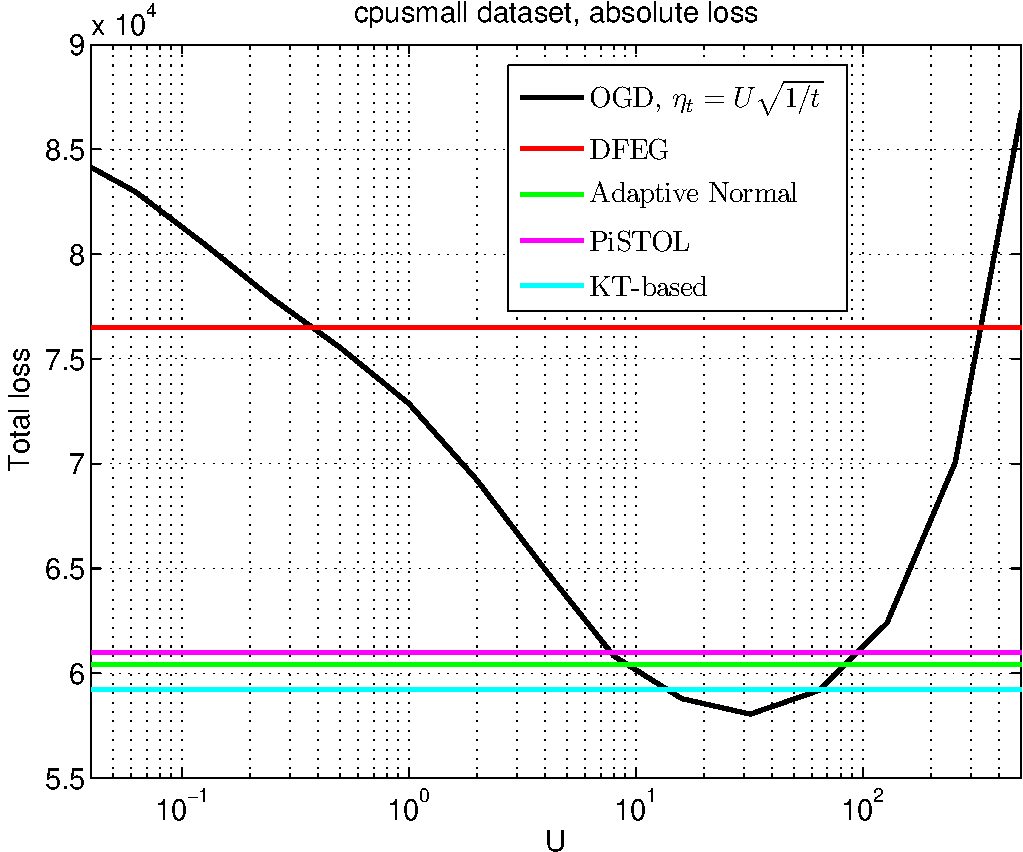
\includegraphics[width=0.32\textwidth]{../NIPS-2016-submission/figs/cpusmall_kt-crop.pdf}}
\subfigure{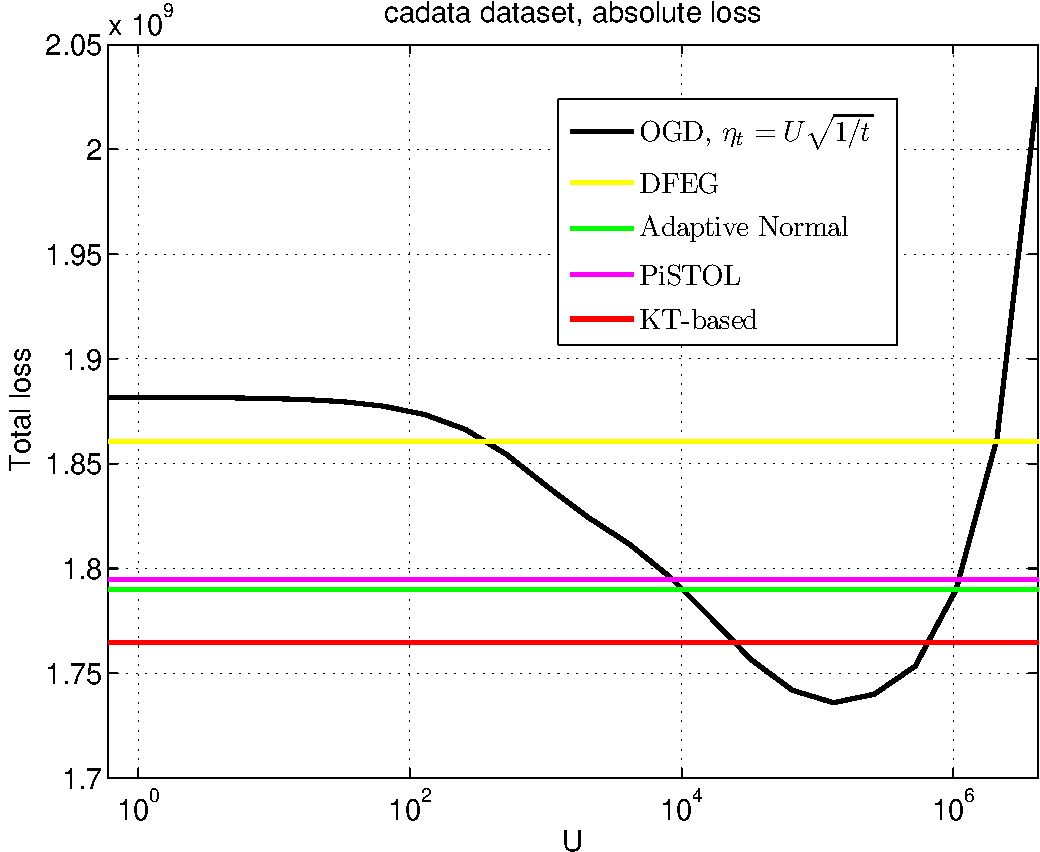
\includegraphics[width=0.32\textwidth]{../NIPS-2016-submission/figs/cadata_kt-crop.pdf}}
\caption{\footnotesize{Total loss versus learning rate parameter of \ac{OGD} (in log scale), compared with parameter-free algorithms DFEG~\cite{Orabona-2013}, Adaptive Normal~\cite{McMahan-Orabona-2014}, PiSTOL~\cite{Orabona-2014} and Algorithm~\ref{algorithm:kt-sgd}.}}
\label{fig:exp_olo}
\end{figure}
